
This chapter presents results of the analysis of cancer data using the
software and algorithms presented in the previous chapter. In section
\ref{sec:analysis_tcgbiolinks} we present some use cases using mainly the TCGAbiolinks
package. In section \ref{sec:analysis_elmer} we present some data analysis using the ELMER package.
In section \ref{sec:glioma_analysis}, using the previous tools described we perfom a
glioma analysis focused specially in the two molecular subtypes G-CIMP-low and
 G-CIMP-high discovered by our laboratory and collaborators.

\section{Use cases using TCGAbiolinks}\label{sec:analysis_tcgbiolinks}

In this section, we introduce and describe the utility and application of TCGAbiolinks
through some use cases.
In subsection  \ref{subsec:analysis_tcgbiolinks2} we show a
lower-grade glioma downstream analysis with gene expression.
In subsection \ref{subsec:analysis_tcgbiolinks3} we show a
downstream analysis integration of gene expression and methylation data of colon
adenocarcinoma data, describing how to generate a starburst plot \cite{noushmehr2010identification},
which was introduced to illustrate the results of integrating
DNA methylation and gene expression data.


\subsection{Lower-grade glioma downstream analysis with gene expression} \label{subsec:analysis_tcgbiolinks2}

For this case study, we used the recently available \sigla{LGG}{lower-grade glioma} data to investigate gene expression differences between the reported molecular subtypes (IDHmutant, IDHwildtype and IDHmutant codels) \cite{platforms2015comprehensive}. In particular, we used TCGAbiolinks to download 293 samples profiled using messenger RNA expression (IlluminaHiSeq RNASeqV2) with available molecular subtypes. The data was normalized using the \textit{TCGAanalyze\_Normalization} function and we applied three filters to remove features/mRNAs with low signals across samples, obtaining 4578, 4284 and 1187 mRNAs, respectively. A clustering analysis was then applied using the ConsensusClusterPlus package \cite{wilkerson2010consensusclusterplus} which identified four distinct groups of samples (EC1-EC4) (Figure \ref{fig:caseexp}A). The survival curves for each cluster were generated using \textit{TCGAanalyze\_survival} and are shown in Figure \ref{fig:caseexp}B. As expected, each cluster effectively separated IDHwildtype tumors (EC1) from IDHmutant-non-codel (EC2) and IDHmutant-codel tumors (EC3 and EC4) (Figure \ref{fig:caseexp}). Additional biological subtypes (DNA methylation subtypes) were reproduced as expected (Figure \ref{fig:caseexp}D) \cite{platforms2015comprehensive}.

\begin{figure*}
\centering
%\includegraphics[width=.9\linewidth]{figures/case3_improved.pdf}
\includegraphics[width=1.0\linewidth]{images/figure4.pdf}
\caption[Case study - LGG downstream analysis with gene expression]{Case study - Integrative (or Downstream) analysis of gene expression and clinical data from LGG disease with unsupervised clustering and crossing expression clusters with clinical and molecular information. \textbf{(A)} Heatmap of 1187 more variables genes clustered with tree $k = 4$ in EC1, EC2, EC3, EC4. \textbf{(B)} Kaplan Meier survivals plot for EC clusters. \textbf{(C and D)} Distribution of the DNA Methylation clusters and ATRX mutation within the EC clusters.}
\label{fig:caseexp}
\end{figure*}

\subsection{Downstream analysis integration of gene expression and methylation data} \label{subsec:analysis_tcgbiolinks3}

The DNA methylation of specific promoter CpG islands has the potential to influence gene expression.
In this case study, we used TCGAbiolinks to examine the biological relationship between DNA methylation
and gene expression in \sigla{COAD}{Colon adenocarcinoma}. Using \textit{GDCquery}, \textit{GDCdownload}
and \textit{GDCprepare}, we obtained DNA methylation data (Infinium HumanMethylation450 and Infinium
HumanMethylation27 platforms) and gene expression data (IlluminaGA RNASeqV2 platform) for the same
TCGA COAD samples \cite{cancer2012comprehensive}. A supervised analysis was performed on the molecular
subtypes CIMP-Low [CIMP.L] and CIMP-High [CIMP.H].
The gene expression analysis started by the identification of outliers, followed by the normalization methods.
 Using \textit{TCGAanalyze\_DEA}, 34 DEGs ($log_2FC\geq 3.0$ and FDR $\leq 10^{-4}$) were identified.
 The result of this analysis is represented in a volcano plot (Figure \ref{fig:case_starburst}A)
 created using \textit{TCGAVisualize\_volcano}.
For the DNA methylation analysis,
using \textit{TCGAanlayze\_DMR} we identified 73 CpG-methylated probes ($\Delta\overline{\beta}\geq 0.25$ and  $FDR \leq 10^{-5}$;  (Figure \ref{fig:case_starburst}B). The DNA methylation and gene expression results were integrated as in the previous TCGA marker paper \cite{noushmehr2010identification,cancer2012comprehensive}, by generating a starburst plot (Figure \ref{fig:case_starburst}C) in which the x-axis is the $log_{10}$ of the correct P-value for DNA methylation and the y-axis is the $log_{10}$ of the correct P-value for the expression data.
The starburst plot highlights nine distinct quadrants.
To incorporate the DNA methylation difference cut-off into the  graph,
we highlighted genes that might have the potential for silencing due to epigenetic alterations.
 We highlighted five genes, EYA1, SIX2, ACSL6, OGDHL and SLC30A2, that showed a $\Delta\overline{\beta}\geq0.25$
 and a $log_2FC\geq 3.0$ between CIMP.L and CIMP.H.

\begin{figure*}
\centering
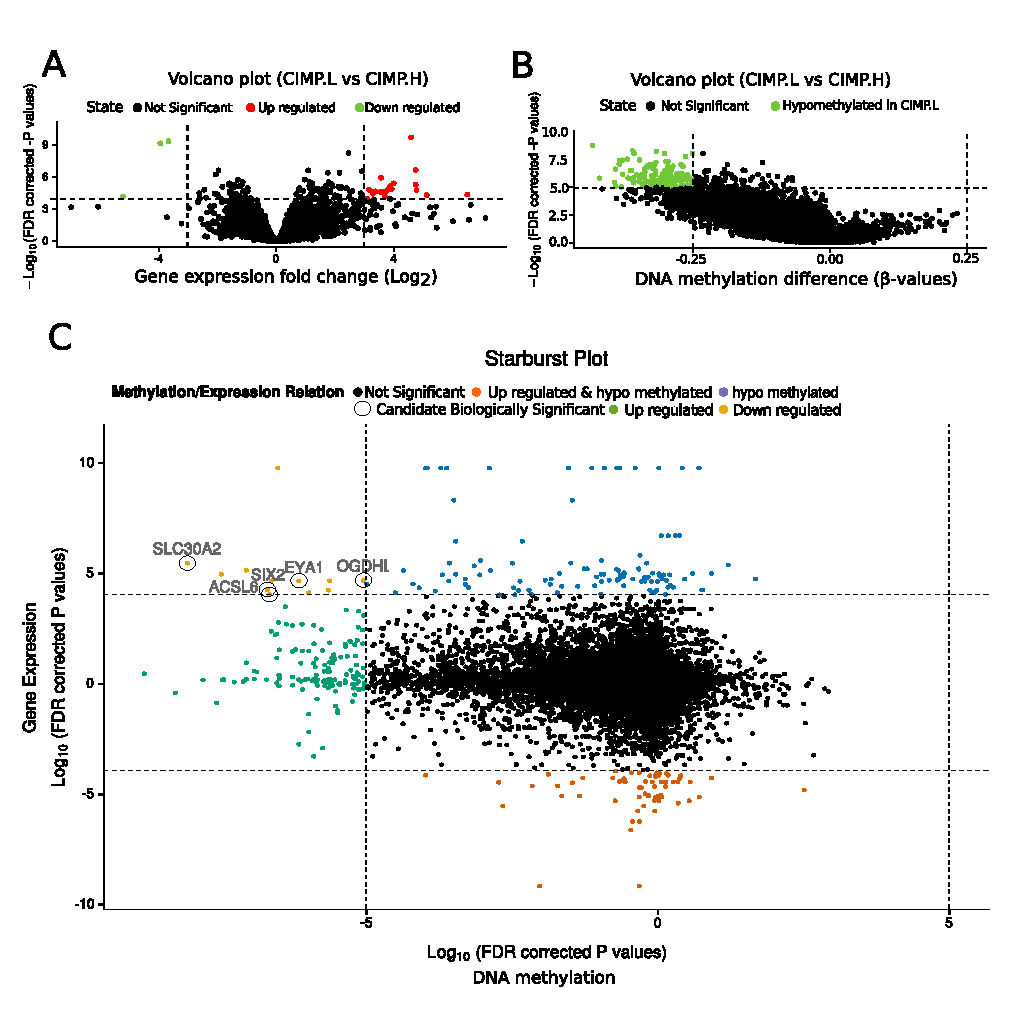
\includegraphics[width=1.0\linewidth]{images/figure5.pdf}
\caption[Case study - Integrative data analysis of Colon Adenocarcinoma]{
Case study - Integrative analysis of gene expression and DNA methylation data from COAD disease,
comparing groups CIMP.L and CIMP.H. \textbf{(A)} Expression volcano plot: fold change of expression data versus significance.
 \textbf{(B)} DNA methylation volcano plot: difference of DNA methylation versus significance.
 \textbf{(C)} Starburst plot: DNA methylation significance versus gene expression significance.}
\label{fig:case_starburst}
\end{figure*}


\section{Use cases using ELMER}\label{sec:analysis_elmer}

%\newpage
\subsection{Use Case 1: Breast Invasive Carcinoma (Unsupervised mode)} 

In this subsection, we describe how to perform \textit{ELMER} analysis on TCGA BRCA
(Breast Invasive Carcinoma) data retrieved from the GDC server.
We first describe how the data can be downloaded and organized to
the default \textit{ELMER} input, followed by the following analysis steps:
\begin{itemize}
	\item Identification of distal probes with significant differential DNA methylation (i.e. DMCs) in tumor vs. normal samples
	\item Identification of putative target gene(s) for differentially methylated distal probes
  \item Characterization of chromatin state context of significant probe regions using FunciVar
	\item Identification of enriched motifs within set of probes in significant probe-gene pairs
	\item Identification of master regulator Transcription Factors (TF) for each enriched motif
\end{itemize}

In addition to these standard steps, we also compared the
putative probe-gene pairs to those derived from deep-sequenced ChIA-PET
data from MCF7 cells (as shown in \citeonline{yao2015inferring}).

\subsubsection*{Downloading TCGA data}

The function \textit{getTCGA} uses the   \href{http://bioconductor.org/packages/TCGAbiolinks/}{TCGAbiolinks}
package \cite{colaprico2015tcgabiolinks} to download TCGA data for all samples
for a given disease (such as BLCA, LGG, GBM). Its main arguments are
the \textit{genome}  that if set to "hg19" will download data from GDC legacy archive, and if set
to "hg38" it will download data from the main GDC harmonized data portal.


%\begin{codigo}[language=R, style = mystyle,label = "download",caption = "Step 1: Downloading TCGA data from GDC database"]
%\end{codigo}

If the \textit{getTCGA} function called before was successful it will
 create the following objects and folders:
\begin{verbatim}
--- DATA/BRCA/
  |----------- BRCA_meth_hg38.rda (object with DNA methylation)
  |----------- BRCA_RNA_hg38.rda (object with gene expression)
  |----------- BRCA_clinic.rda   (object with indexed clinical information)
  |----------- Raw/ (folder: contains All raw data from GDC)
\end{verbatim}

\subsubsection*{Selecting distal probes}

The function \textit{get.feature.probe}, shown in Listing \ref{lst:distal},
is used to select HM450K/EPIC probes located away from any TSS (at least $2Kb$ away).
Its main arguments are the genome of reference ("hg38"/"hg19") and DNA methylation
platform ("450K"/"EPIC"). The \textit{feature} argument is used to limit the region of probes; as we want all distal probes, we set it to NULL.
%Later, we will use all distal probes and annotate their chromatin state later with
%MCF-7 annotation tracks from the NIH Roadmap Epigenomics Mapping Consortium \cite{bernstein2010nih}  available at StateHub (\url{http://statehub.org/})\cite{Coetzee127720}.

\lstinputlisting[language=R,basicstyle=\tiny, frame = none, label = {lst:distal},caption = "Selection of probes within biofeatures"]{codes/distal_probes.R}

\subsection*{Organizing data into a MultiAssayExperiment object}
The function \textit{createMAE} is used to organize the gene expression and
 DNA methylation data into a MultiAssayExperiment (MAE) object. Listing \ref{lst:mae}
 shows how to use it with the data created in the previous steps.
  Its main arguments are described below:

\begin{itemize}
\item \textit{exp} : An R object or a path to a file containing a gene expression
    matrix or SummarizedExperiment with gene counts.
\item \textit{met} : An R object or a path to a file containing a DNA methylation
    matrix or SummarizedExperiment with beta values.
\item \textit{met.platform}: DNA methylation platform.
    "EPIC" for Infinium MethylationEPIC or "450K" for
    Infinium HumanMethylation450.
 \item \textit{genome}: The genome of reference ("hg19" or "hg38")
    used to select the correct metadata. Genes genomic ranges will be annotated
    using ENSEMBL database and DNA methylation probes
    using metadata available at \url{http://zwdzwd.github.io/InfiniumAnnotation}.
 \item \textit{linearize.exp}: this step will take the $log_2(gene\; expression + 1)$
    in order to linearize the relationship between
    gene expression and DNA methylation.
 \item \textit{filter.probes}: genomic ranges (i.e. distal
    regions) within which  probes from
    DNA methylation data should be kept.
 \item \textit{met.na.cut}: maximum percentage of empty values (NA) a probe might have to be
    considered in the analysis. The default is 20\% (i.e if 50\% of samples has empty values  for a given
    probe, it will be removed).
 \item \textit{colData}: A matrix  with samples metadata (i.e. clinical data ,
    molecular  subtype information). If argument TCGA is set to \textit{TRUE}
    this matrix will be created automatically. In this case, the \textit{colData}
    argument is optional.
 \item \textit{sampleMap}: A matrix mapping DNA methylation data and gene expression
    data to samples. \textit{ELMER} uses only samples with both data.
    Otherwise,  it will be removed. If argument TCGA is set to \textit{TRUE}
    this matrix will be created automatically. In this case \textit{sampleMap}
    argument is optional.
\end{itemize}

\lstinputlisting[language=R,basicstyle=\tiny, frame = none, label = {lst:mae},caption = "Create MultiAssayExperiment"]{codes/mae.R}

Listing \ref{lst:verifymae} shows information about the object created.
There are 866 samples with both gene expression and DNA methylation data,
and among those 5 are metastatic samples, 778 are Primary Solid Tumor and
83 are Solid Tissue Normal.

\lstinputlisting[language=R,basicstyle=\tiny, frame = none, label = {lst:verifymae},caption = "Verifying MultiAssayExperiment"]{codes/mae_verify.R}


\subsubsection*{Identification of distal probes with significant differential DNA methylation (i.e. DMCs) in tumor vs. normal samples}

The function \textit{get.diff.meth} is  used to identify regions differentially methylation between two groups.
Listing \ref{lst:diffMeth} shows how to use it to select hypomethylated probes in "Primary solid tumor" samples
when compared to "solid tissue normal" samples  ($FDR \leq 0.01$, $\Delta\overline{\beta}\geq 0.3$), using those samples
in the lower quintile ($minSubgroupFrac = 0.2$) of DNA methylation levels for each probe.
Its main arguments are described below:


\begin{itemize}
\item \textit{data} A multiAssayExperiment with DNA methylation and Gene Expression data.
\item  \textit{group.col}	A column defining the groups of the sample. You can view the available columns using: colnames(MultiAssayExperiment::colData(data)).
\item  \textit{group1}	A group from group.col. \textit{ELMER} will run group1 vs group2. That means, if the direction is hyper, get probes hypermethylated in group 1 compared to group 2.
\item  \textit{group2}	A group from group.col. \textit{ELMER} will run group1 vs group2. That means, if the direction is hyper, get probes hypermethylated in group 1 compared to group 2.
\item \textit{diff.dir} Differential methylation direction. It can be "hypo" which is only selecting hypomethylated probes in group 1 when compared to group 2; "hyper" which is only selecting hypermethylated probes;
\item  \textit{minSubgroupFrac} A number ranging from 0 to 1, specifying the fraction of extreme samples from group 1 and group 2 that are used to identify the differential DNA methylation. The default is 0.2 because we typically want to be able to detect a specific (possibly unknown) molecular subtype among tumor; these subtypes often make up only a minority of samples, and 20\% was chosen as a lower bound for the purposes of statistical power. If you are using pre-defined group labels, such as treated replicates vs. untreated replicated, use a value of 1.0 (\textit{Supervised} mode)

\item  \textit{pvalue} A number specifying the significant P value (adjusted P value by Benjamini-Hochberg procedure) cutoff for selecting significant hypo/hyper-methylated probes. The default is 0.01.
\item  \textit{sig.dif} A number specifying the smallest DNA methylation difference as a cutoff for selecting significant hypo/hyper-methylated probes. The default is 0.3.
\end{itemize}

%\begin{minipage}{\linewidth}
\lstinputlisting[language=R,basicstyle=\tiny, frame = none, label = {lst:diffMeth},caption = "Identify significantly different DNA methylation probes in tumor and normal samples"]{codes/diffMeth.R}
%\end{minipage}

If the \textit{save} argument is set to TRUE, in the \textit{dir.out} folder two files will be created: \textit{getMethdiff.hypo.probes.csv} containing all probes from the DNA methylation data with the difference means of the groups and the significance values, \textit{getMethdiff.hypo.probes.significant.csv} will contain only probes that respect the thresholds. Table \ref{tab:diff.meth} shows the first rows of  \textit{getMethdiff.hypo.probes.significant.csv} file.

\begin{table}[h!]
\csvautobooktabular[respect underscore,
                    filter expr={test{\ifnumless{\thecsvinputline}{5}}}]{tables/getMethdiff.hypo.probes.significant.csv}
\caption[Identification of distal probes with significant differential DNA methylation (i.e. DMCs)]{Identification of distal probes with significant differential DNA methylation (i.e. DMCs): First three rows of  getMethdiff.hypo.probes.significant.csv file. }
\label{tab:diff.meth}
\end{table}

\newpage
\subsubsection*{Identification of putative target gene(s) for differentially methylated distal probes}
The function \textit{get.pair} is used to link enhancer probes with methylation changes to target genes with expression changes and report the putative target gene for selected probes. Listing \ref{lst:getpair} shows how to select the 20 nearest genes (10 downstream and 10 upstream) and evaluate if each pair is anti-correlated (probes with higher methylation levels have lower gene expression levels).
Its main arguments are described below:

\begin{itemize}
\item \textit{nearGenes:} Output of \textit{GetNearGenes} function.
\item  \textit{mode:} Algorithm mode: "unsupervised" or "supervised". If unsupervised is set
the $U$ (unmethylated) and $M$ (methylated) groups will be selected
among all samples of both groups based on methylation of each probe.
Otherwise $U$ group and $M$ group will set as all the samples of group1 or group2 as described below:
If diff.dir is "hypo, $U$ will be the group 1 and $M$ the group2.
If diff.dir is "hyper" $M$ group will be the group1 and $U$ the group2.
\item \textit{minSubgroupFrac:} A number ranging from 0 to 1, specifying the fraction of extreme  samples that define group U (unmethylated) and group M (methylated), which are used to link probes to genes. The default is 0.4 (the lowest quintile of samples is the U group and the highest quintile samples is the M group) because we typically want to be able to detect a specific (possibly unknown) molecular subtype among tumor; these subtypes often make up only a minority of samples, and 20\% was chosen as a lower bound for the purposes of statistical power. This argument is Only used if mode is "supervised", otherwise if you are using pre-defined group labels ("supervised" mode), such as treated replicates vs. untreated replicated, it will use all samples.
\item  \textit{permu.size:} Number of permutation. The default is $10000$. \textit{Note}: This parameter can strongly impact run time.
\item \textit{raw.pvalue:} Raw p-value cutoff for defining significant pairs. The default is $0.001$.
\item \textit{Pe:} Empirical p-value cutoff for defining significant pairs. The default is $0.001$.
\item \textit{filter.probes:} Should probes be filtered  by selecting only those which have at least a certain number of samples below and above a certain cut-off ? If true, arguments \textit{filter.probes} and \textit{filter.percentage} will be used.
\item  \textit{filter.portion:}	A number specifying the cut point to define binary methylation level for probe loci. The default is 0.3. When the beta value is above 0.3, the probe is methylated and vice versa. For one probe, the percentage of methylated and unmethylated samples should be above filter.percentage value. Only used if \textit{filter.probes} is TRUE.
\item  \textit{filter.percentage:}	Minimum percentage of samples to be considered in methylated and unmethylated for the filter.portion option. Default 5\%. Only used if \textit{filter.probes} is TRUE.
\end{itemize}


\lstinputlisting[language=R,basicstyle=\tiny, frame = none, label = {lst:getpair}, caption = "Identify putative target genes for differentially methylated distal probes"]{codes/getpair.R}

The output of this function is shown in table \ref{tab:get.pair}. Probe and GeneID
columns show the significant pair and the column $P_e$ shows the adjusted p-value.
\begin{table}[h!]
\centering
\small
\csvautobooktabular[respect underscore,
					before reading=\sisetup{round-mode=places,round-precision=2},
                    filter expr={test{\ifnumless{\thecsvinputline}{5}}}]{tables/getPair.hypo.pairs.significant.csv}
\caption [Identification of putative target gene(s) for differentially methylated distal probes]{
Identification of putative target gene(s) for differentially methylated distal probes: First three rows of  getPair.hypo.pairs.significant.csv file.
}
\label{tab:get.pair}
\end{table}

To visualize the relationship between the probe-gene pairs inferred, there are two auxiliary functions in ELMER. The function \textit{schematic.plot}, shown in Listing \ref{lst:plotpair}, which will plot genes and probes in a specified genomic region, highlighting the significant pairs identified by plotting a genomic interactions track and highlight the genes in the pair in red (Figure \ref{fig:pairplot}). Also,  using the function \textit{scatter.plot} (Listing \ref{lst:scatterplot}) it is possible to visualize the correlation between gene expression and DNA methylation levels at probe (Figure \ref{fig:scatterplot}).
 Finally, an overall summary of the DNA  methylation levels and gene expression levels  can be visualized using the auxiliary function \textit{heatmapPairs}, as shown in Listing \ref{lst:heatmap}. This function creates a heatmap for all samples  as shown in Figure \ref{fig:heatmap}.

%\begin{minipage}{\linewidth}
\lstinputlisting[language=R,basicstyle=\tiny, frame = none,firstline=5,lastline=13,label = {lst:plotpair},caption = "Schematic plot to visualize gene-probe pairs"]{codes/plotpair.R}
%\end{minipage}

\begin{figure}
\centering
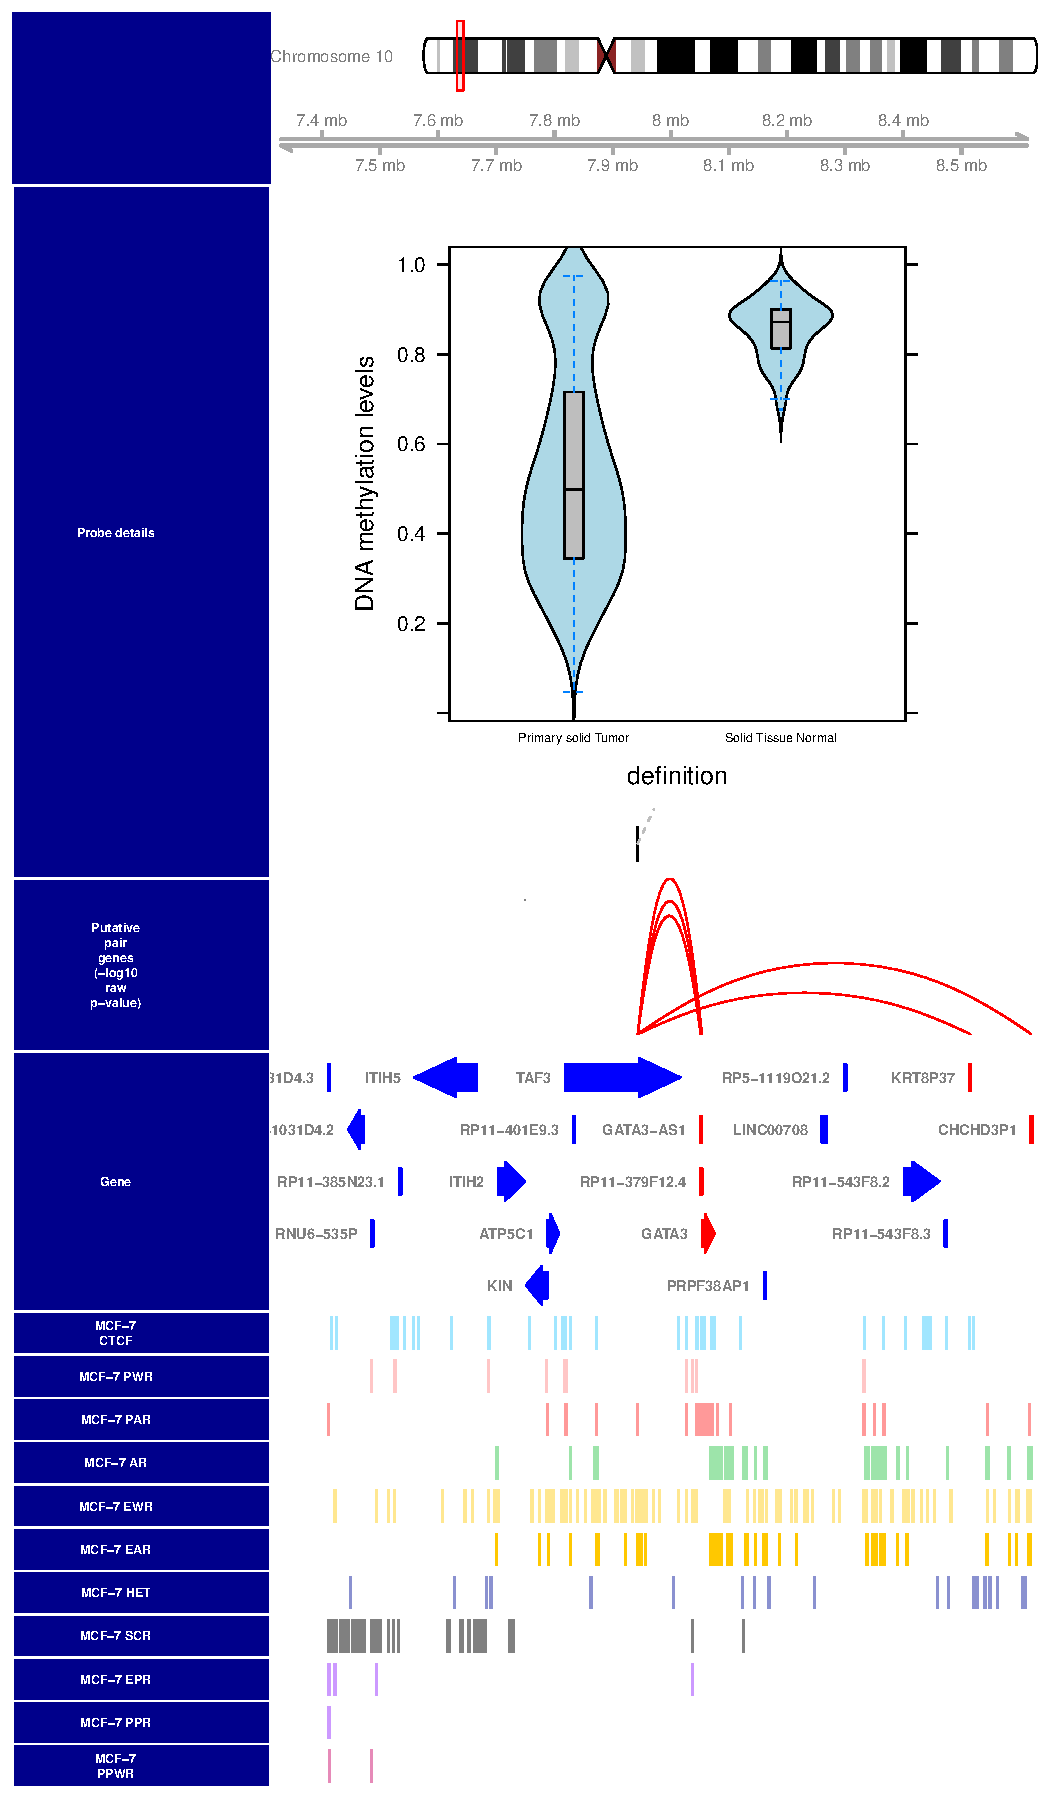
\includegraphics[width=0.7\textwidth]{images/cg04723436_schematic_byProbe.pdf}
\caption[Schematic plot gene-probe pairs]{\label{fig:pairplot} Plot probe-gene pairs with annotation track for MCF-7 cell line from \url{StateHub.org}. Significant probes and gene pairs are highlighted in red.}
\end{figure}

\lstinputlisting[language=R,basicstyle=\tiny, frame = none,label = {lst:scatterplot},caption = "Scatterplot to visualize correlation between gene expression and DNA methylation levels at probe"]{codes/scatterplot.R}


\begin{figure}
\centering
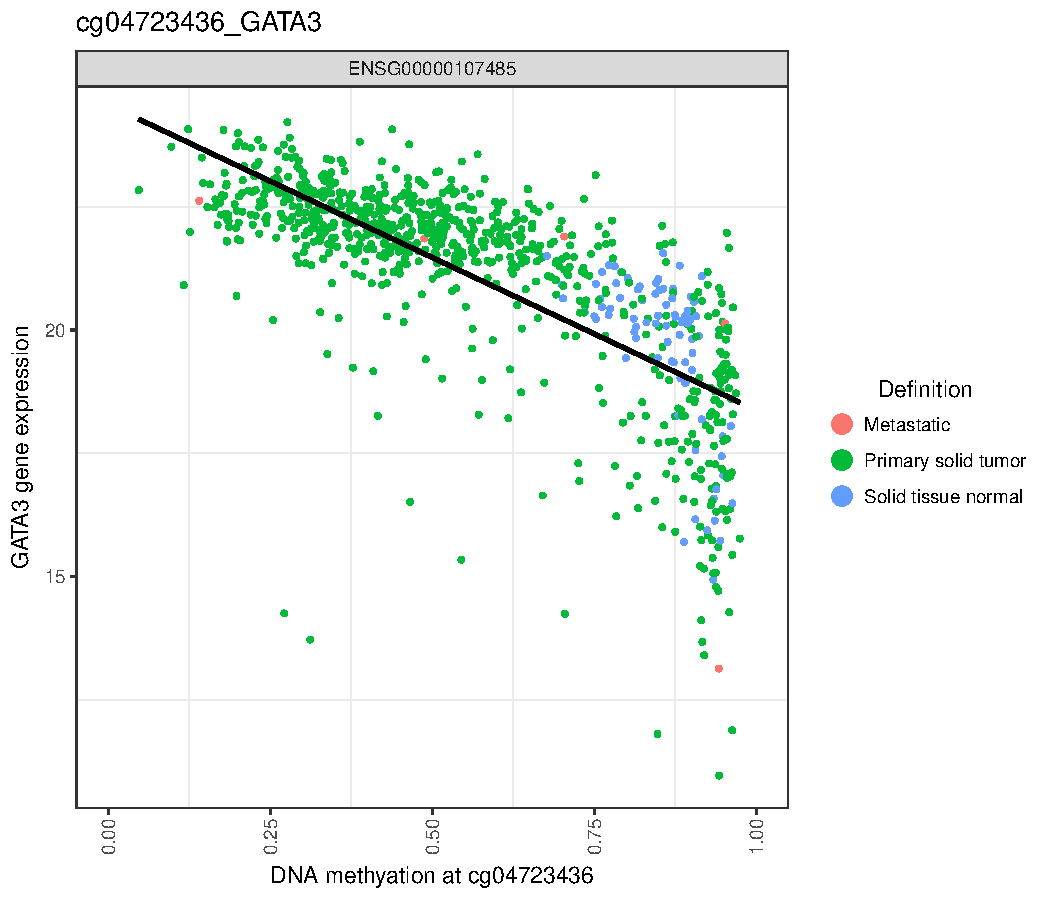
\includegraphics[width=0.7\textwidth]{images/cg04723436_GATA3_bypair.pdf}
\caption{\label{fig:scatterplot} Scatter plot for significant probe (cg04723436) gene (GATA3) pair.}
\end{figure}

\begin{figure}
\centering
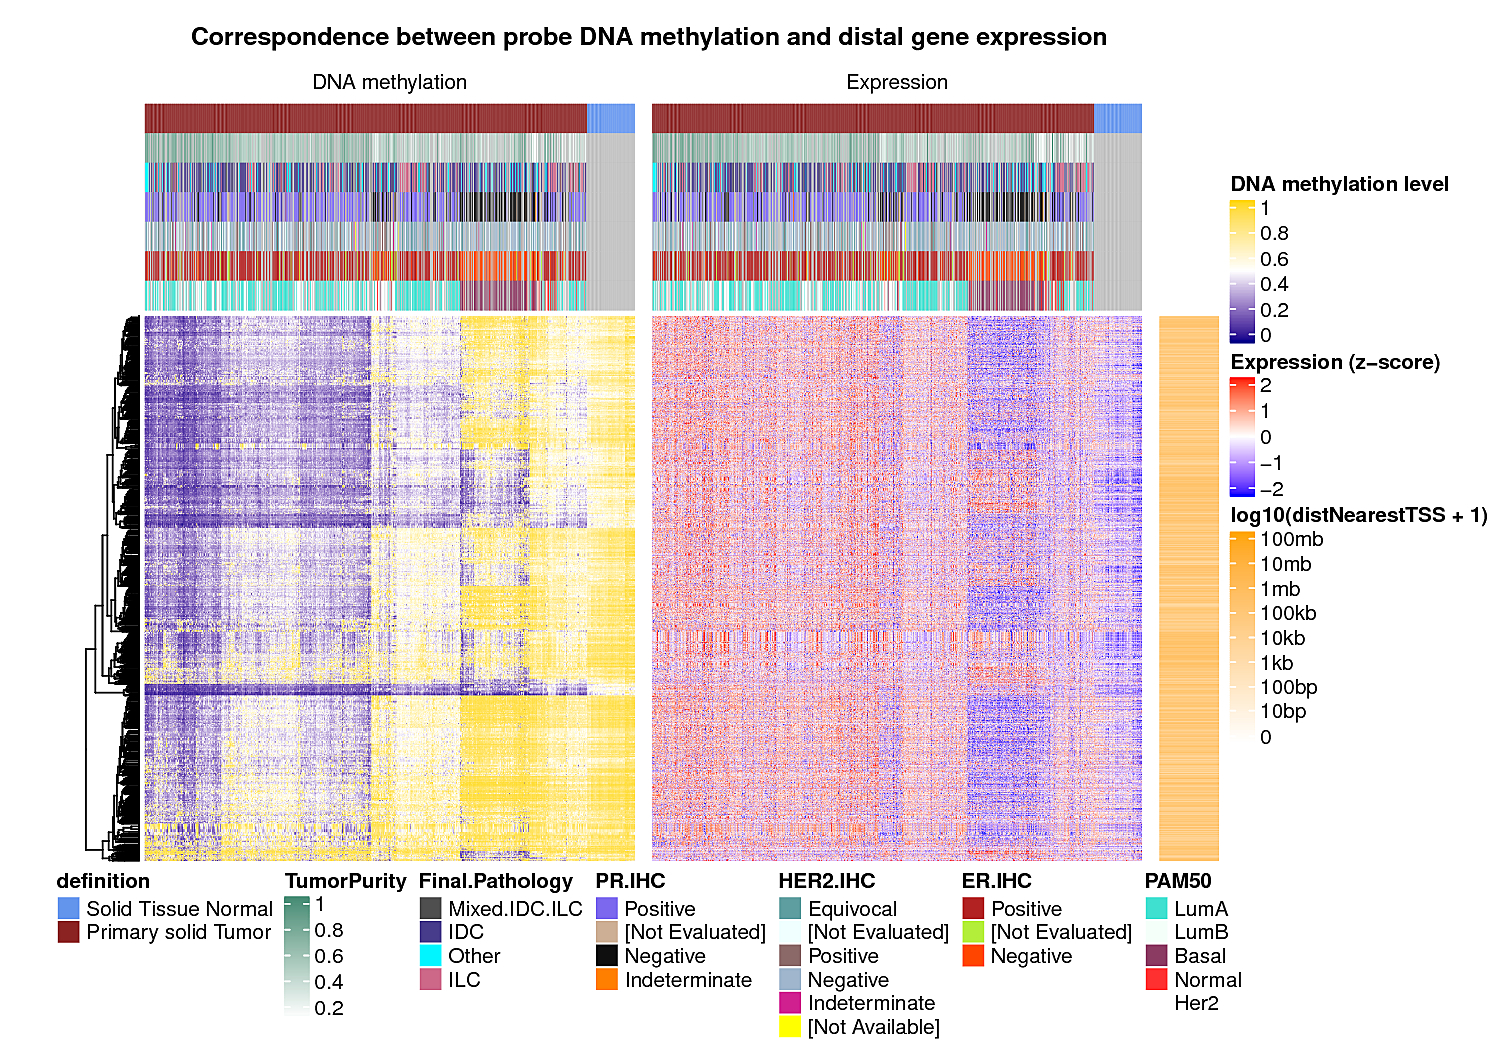
\includegraphics[width=1.0\textwidth]{images/heatmap.jpg}
\caption{\label{fig:heatmap} The comprehensive heatmap view shows all probe / gene pairs identified by ELMER, clustered according to similarity. This plot is based on the Supervised analysis of LumA vs Basal-like Breast Cancer cases. The inverse correlation between methylation and expression can be observed.}
\end{figure}

\clearpage
\lstinputlisting[language=R,basicstyle=\tiny,frame = none,label = {lst:heatmap},caption = "Heatmap to visualize gene-probe pairs"]{codes/heatmap.R}

\clearpage

\subsubsection*{Characterization of chromatin state context of significant probe regions using FunciVar}

To understand and compare our set of probes identified in the probe-gene pairs inferred
we used chromatin state of IHEC cell types
from \url{http://statehub.org/}, to calculate the relative enrichment of
different states.
This procedure uses code from the statepaintR \cite{statepaintr} and FunciVar \cite{funcivar} packages.
Figure \ref{fig:funcivar} shows the enrichment for 14 encode cells lines.
The plot shows enrichment for enhancer active region (EAR), weak enhancer (EWR)
and active promoter region (PAR) in MCF-7 cell (human breast adenocarcinoma cell line)
while for other cell lines this enrichment is not visible.

% https://www.ebi.ac.uk/training/online/course/functional-genomics-introduction-embl-ebi-resource/what-functional-genomics-1
%The functional genomics studies investigates a range of processes such as transcription, translation and epigenetic regulation to understand the complex relationship between genotype and phenotype. Among the main issues it tries to elucidate, we can mention  understanding of the regulation of the genes, finding the active gene promoters in a particular cell type and identifying the functional roles of different genes.
%In view of these questions, several international consortia emerged whose objectives could help clarify some of these issues.
%As examples of these consortia we can cite ENCODE (Encyclopedia of DNA Elements) whose objective was to create a comprehensive catalog of candidate functional elements in the genome and REMC (the Roadmap Epigenomics Mapping Centers project), whose objective was to generate reference epigenomic maps for “normal” human cells/tissues.

%These consortia made available a large amount of data such as transcription, transcription factor binding, histone modifications, DNase hypersensitivity, DNA methylation, DNA-DNA interactions, and RNA-protein interactions that have been used to  annotate chromatin state. Listing shows how to use MCF-7 annotation tracks from \url{http://statehub.org/}  to annotate chromatin state of those pairs identified previously.  (see Additional file for the code

%\begin{minipage}{\linewidth}
%\lstinputlisting[language=R,basicstyle=\tiny, frame = none,basicstyle=\ttfamily\scriptsize]{codes/enhancer.R}
%\end{minipage}
%\begin{minipage}{\linewidth}
%\lstinputlisting[language=R,basicstyle=\tiny, frame = none,basicstyle=\ttfamily\scriptsize,label = {lst:funcivar},caption = "Chromatin state annotation for probe regions"]{codes/funcivar.R}
%\end{minipage}

\begin{figure}
\centering
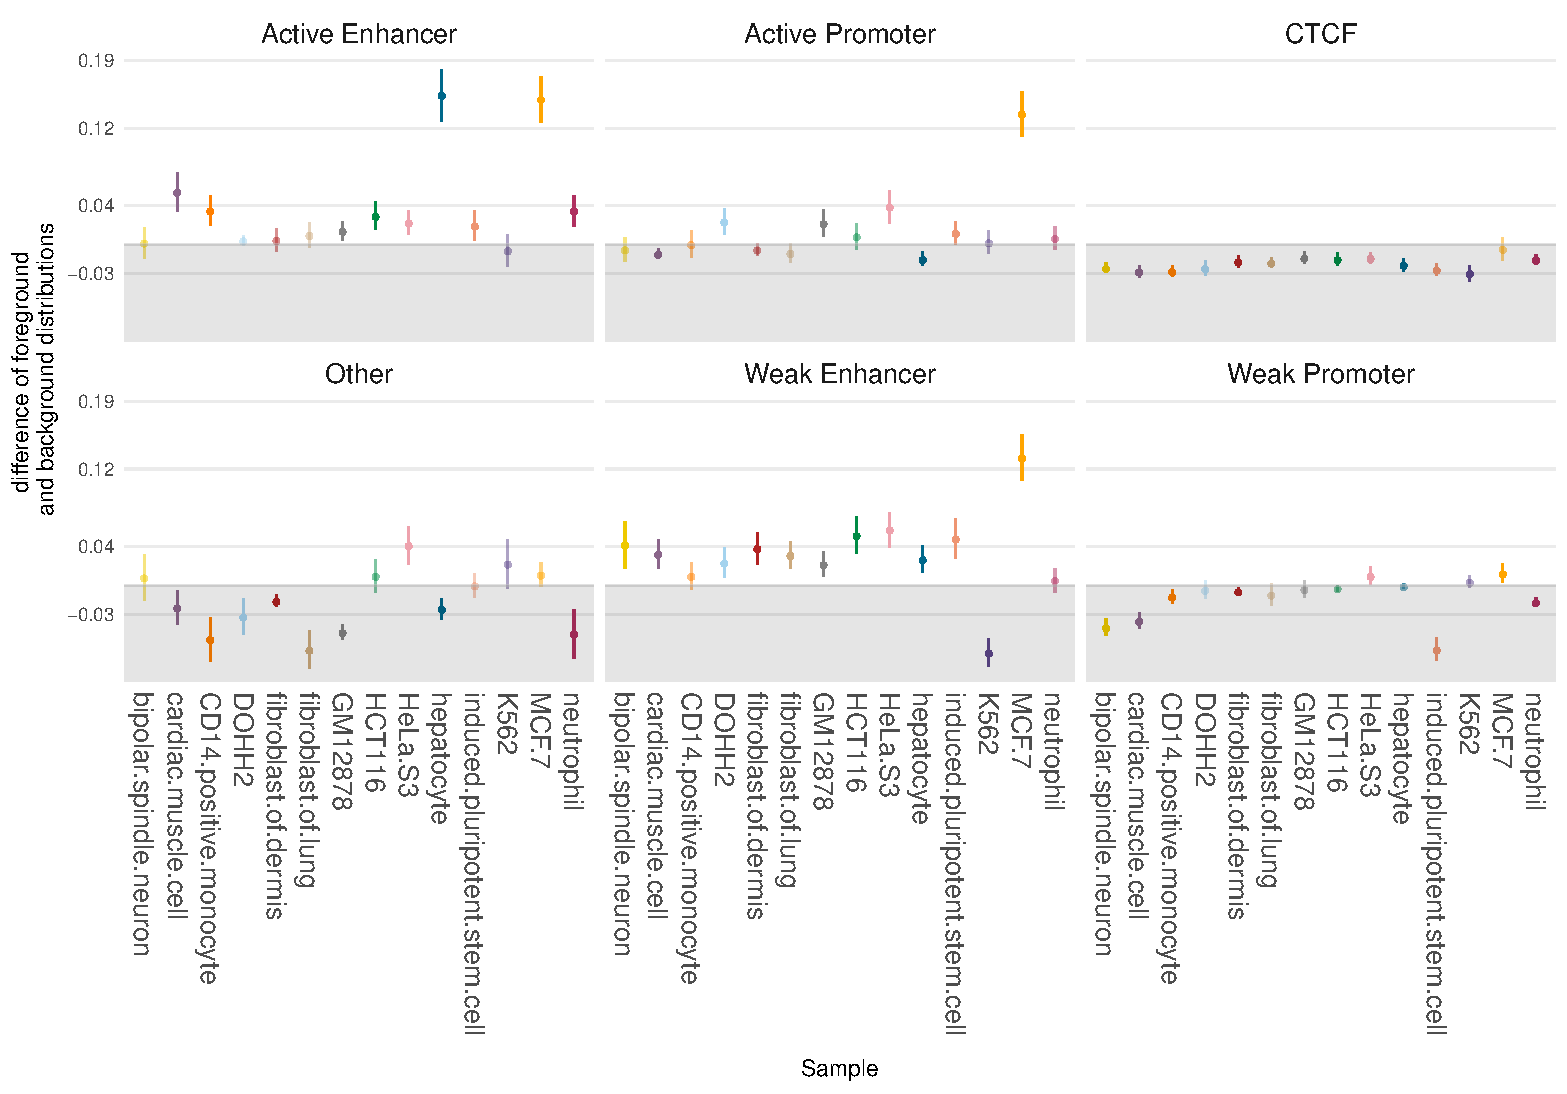
\includegraphics[width=1.0\textwidth]{images/funcivar.pdf}
\caption[ Enrichment of paired probes and chromatin states of encode cells.]{\label{fig:funcivar} Enrichment of paired probes and chromatin states of encode cells.
The plot shows enrichment for enhancer active region, weak enhancer  and active
promoter region for MCF-7 cell. Acronyms - AR: Active region, EAR: active enhancer,
 EWR: Weak Enhancer, EPR: poised enhancer, PAR: active promoter, PWR: Weak Promoter,
 PPR: poised promoter, PPWR: Weak Poised Promoter, CTCF: architectural complex,
 TRS: transcribed, HET: heterochromatin, SCR: Polycomb Repressed Silenced}
\end{figure}


%\cleardoublepage

\subsubsection*{Identification of enriched motifs within set of probes in significant probe-gene pairs}
The function \textit{get.enriched.motif} is used to identify enriched motif in a set of probes.
The main arguments are described below:
\begin{itemize}
\item \textit{lower.OR}	 The motif with lower boundary of 95\% confidence interval for Odds Ratio $\geq lower.OR$  are the significantly enriched motifs.
\item \textit{min.incidence} Minimum number of probes having the motif signature (default: 10) required for a motif to be enriched.
\end{itemize}

%\begin{minipage}{\linewidth}
\lstinputlisting[language=R,basicstyle=\tiny, frame = none,label = "motif",caption = "Motif enrichment analysis on the selected probes"]{codes/motif.R}
%\end{minipage}

\begin{figure}
\centering
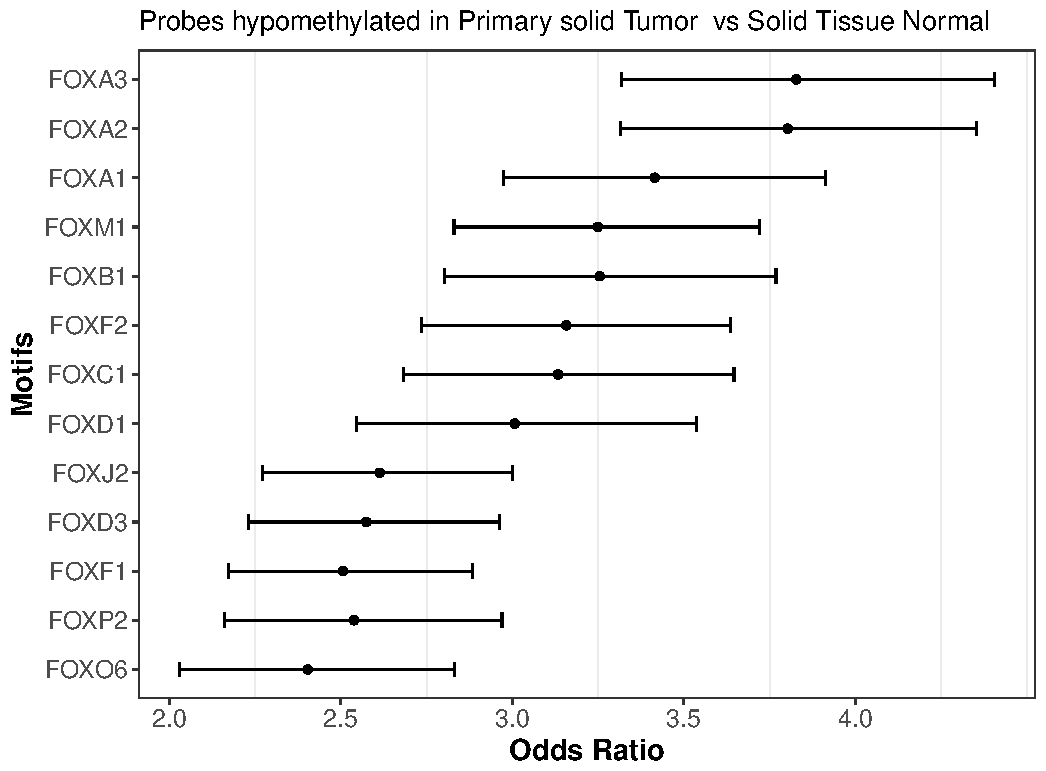
\includegraphics[width=1.0\textwidth]{images/motif_new.pdf}
\caption{\label{fig:motifplot} Motif enrichment plot shows the enrichment levels ($OR\geq2.0$) for the most significant motifs based on the TCGA Breast Cancer Unsupervised analysis. A number of less significant motifs meet our default OR threshold of 1.1 ($\textit{lower.or}=1.1$), which can be browsed in our full Supplemental output report.}
\end{figure}

%\cleardoublepage
\subsubsection*{Identification of master regulator Transcription Factors (TF) for each enriched motif}
The function \textit{get.TFs} is used to identify regulatory TF whose expression associates with TF binding motif
DNA methylation which.

\lstinputlisting[language=R,basicstyle=\tiny, frame = none,label = "tf",caption = "Identifying regulatory Transcript Factors"]{codes/tf.R}

The result of this function is shown in table \ref{tab:get.tf} and in figure \ref{fig:tfplot}.

\begin{landscape}

\begin{table}
\centering
\small
\csvautobooktabular[respect underscore,
					before reading=\sisetup{round-mode=places,round-precision=2},
                    filter expr={test{\ifnumless{\thecsvinputline}{20}}}]{tables/getTF.hypo.significant.TFs.with.motif.summary.csv}
\caption[Identification of master regulator Transcription Factors (TF) for each enriched motif] {First twenty rows of  the \textit{getTF.hypo.significant.TFs.with.motif.summary.csv} file created by \textit{get.Tfs} function (suffix "\_HUMAN.H11MO" was removed from motifs names). First column shows the enriched motif, "top\_5percent\_TFs" shows the top 5\% TFs ranked (the same as all TFs to the left of the dashed line in figure \ref{fig:tfplot}), "potential.TFs.family" are the TF from the "top\_5percent"  that belongs to the same family as the TF of the motif, "top.potential.TFs.family" is the highest ranked TF belonging to the same family as the TF of the motif (same as the first TF from "potential.TFs.family" column). The columns "potential.TFs.subfamily" and "top.potential.TFs.subfamily" are the same as "potential.TFs.family" and "top.potential.TFs.family"  but considering the subfamily classification instead. For example, the motif ANDR has two TFs in the top 5\% that belongs to the same TF family (Steroid hormone receptors): ESR1 and AR, but if considering subfamilies only AR in considered.
}
\label{tab:get.tf}
\end{table}
\end{landscape}


\begin{figure}
\centering
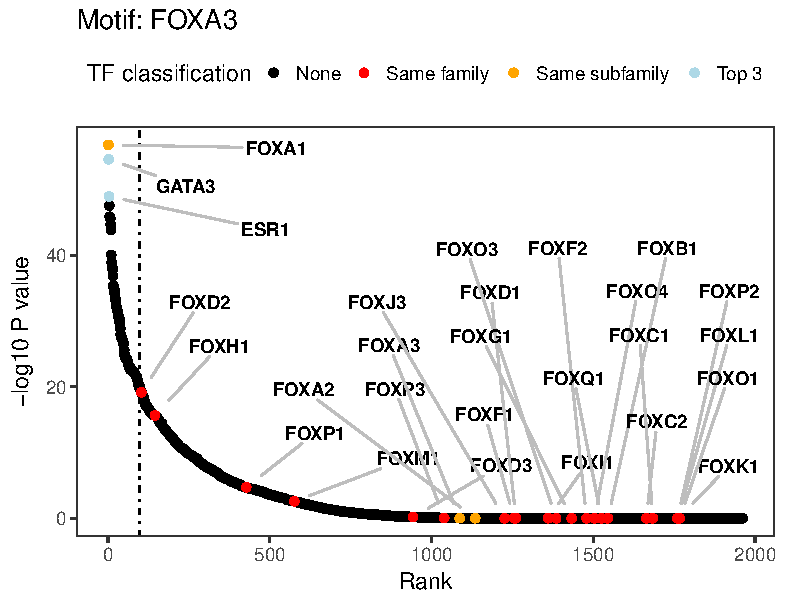
\includegraphics[width=0.9\textwidth]{images/TFranking.pdf}
\caption{\label{fig:tfplot} TF ranking plot shows the statistical $-log_{10}(P-value)$ assessing the anti-correlation level of candidate Master Regulator TF expression with average DNA methylation level for sites with the given motif (FOXA3). By default, the top 3 associated TFs (blue dots), and all of the TF family members (red dots) and subfamily members (orange dots) are labeled. The anti-correlation data for the top three candidates (FOXA1, GATA3, and ESR1) are derived from the data shown in Figure \ref{fig:scatter}}
\end{figure}

\begin{figure}
\centering
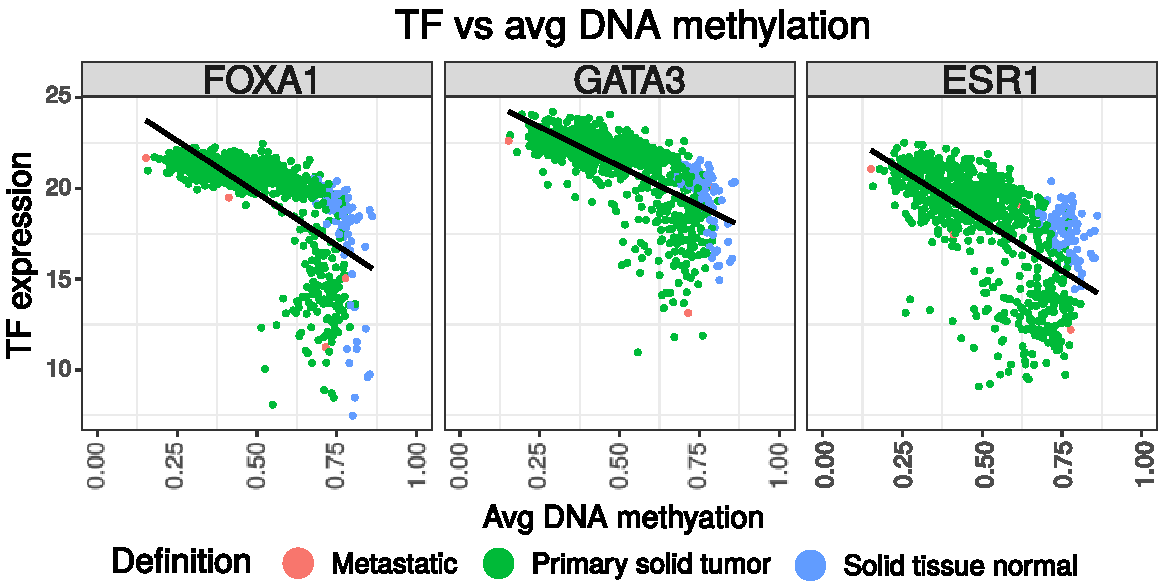
\includegraphics[width=1.0\textwidth]{images/scatter_font.pdf}
\caption{\label{fig:scatter} FOXA1, GATA3 and ESR1 were identified as the most significant Master Regulator candidates for the top motif (FOXA3). All FOX factors belonging to the same TFClass binding family are highlighted.}
\end{figure}

%\clearpage


\subsubsection*{Comparing inferred results with MCF-7 chIA-PET}

As shown in \citeonline{yao2015inferring}, we compared the putative pairs inferred to the chromatin loops derived from deep-sequenced ChIA-PET data from MCF7 cells \cite{li2012extensive}. First, we identify the number of \textit{ELMER} pairs overlapping the ChIA-PET loops, then we repeat using randomly generated  pairs with properties similar to the \textit{ELMER} pairs. For each true ELMER probe in a probe-gene pair, we randomly select a different probe from the complete set of distal probes. We then choose the nth nearest gene to the random probe, where n is the same as the adjacency of the true ELMER probe (i.e. if the true probe is linked to the second gene upstream, the  random probe will also be linked to its second gene upstream). Thus, the random linkage set has both the same number of probes and the same number of linked genes as the true set. One hundred such random datasets were generated to arrive at a 95\% CI ($\pm 1.96* SD$).
The result is shown in Figure \ref{fig:chiapet}. Of the 2124 putative pairs identified in breast cancer tumors, 316 (approximately 14.9\%) were also identified as loops in the MCF7 ChIA-PET data. This was a three-fold enrichment over randomized probe-gene pairs (see Additional file for the code).


\begin{figure}
\centering
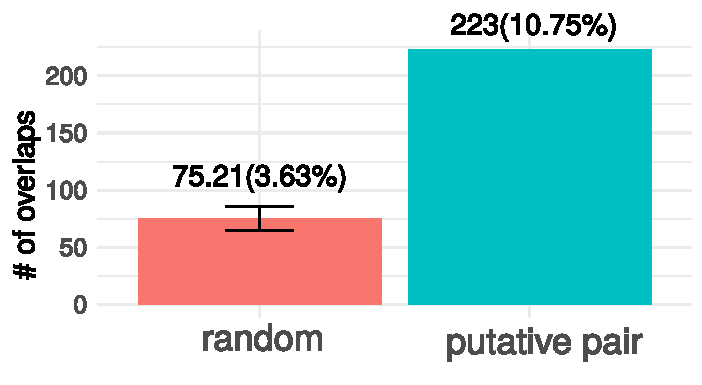
\includegraphics[width=0.5\textwidth]{images/mcf7.pdf}
\caption[MCF7 ChIA-PET validation]{\label{fig:chiapet} The graph shows the comparison of the number of probe-gene pairs identified within MCF7 ChIA-PET data using the putative pairs from BRCA vs. random pairs}
\end{figure}

%\clearpage
\subsection{Use Case 2: BRCA molecular subtypes analysis (Supervised mode)} 


Several studies identified distinct molecular Breast Cancer molecular subtypes including luminal-like (Luminal A and Luminal B) subclasses, which are Estrogen receptor-positive (ER-positive), and the basal-like, ErbB2-positive and normal-like subclasses (ER-negative) \cite{perou2000molecular,yersal2014biological,sorlie2001gene}. We performed \textit{ELMER} analysis comparing known molecular subtypes (Her2, Luminal A, Luminal B and Basal-like) using the TCGA BRCA dataset and classifications retrieved from \cite{ciriello2015comprehensive} using TCGABiolinks.
% TIAGO IS THIS CORRECT?  DID YOU USE BIOLINKS? 
% Yes, the data was downloaded using TCGAbiolionks 
% The annotation was added manually

We performed pairwise analyses between different molecular subtypes. It is important to note that we expect these analyses to have increased statistical power over Unsupervised analyses, as illustrated above in Figure \ref{fig:mode}. One useful output plot is the comprehensive heatmap, 
which illustrates the identification of inverse correlated probe-gene pairs \ref{fig:heatmap} for the LumA vs Basal-like analysis.  

\begin{figure}[ht!]
\centering
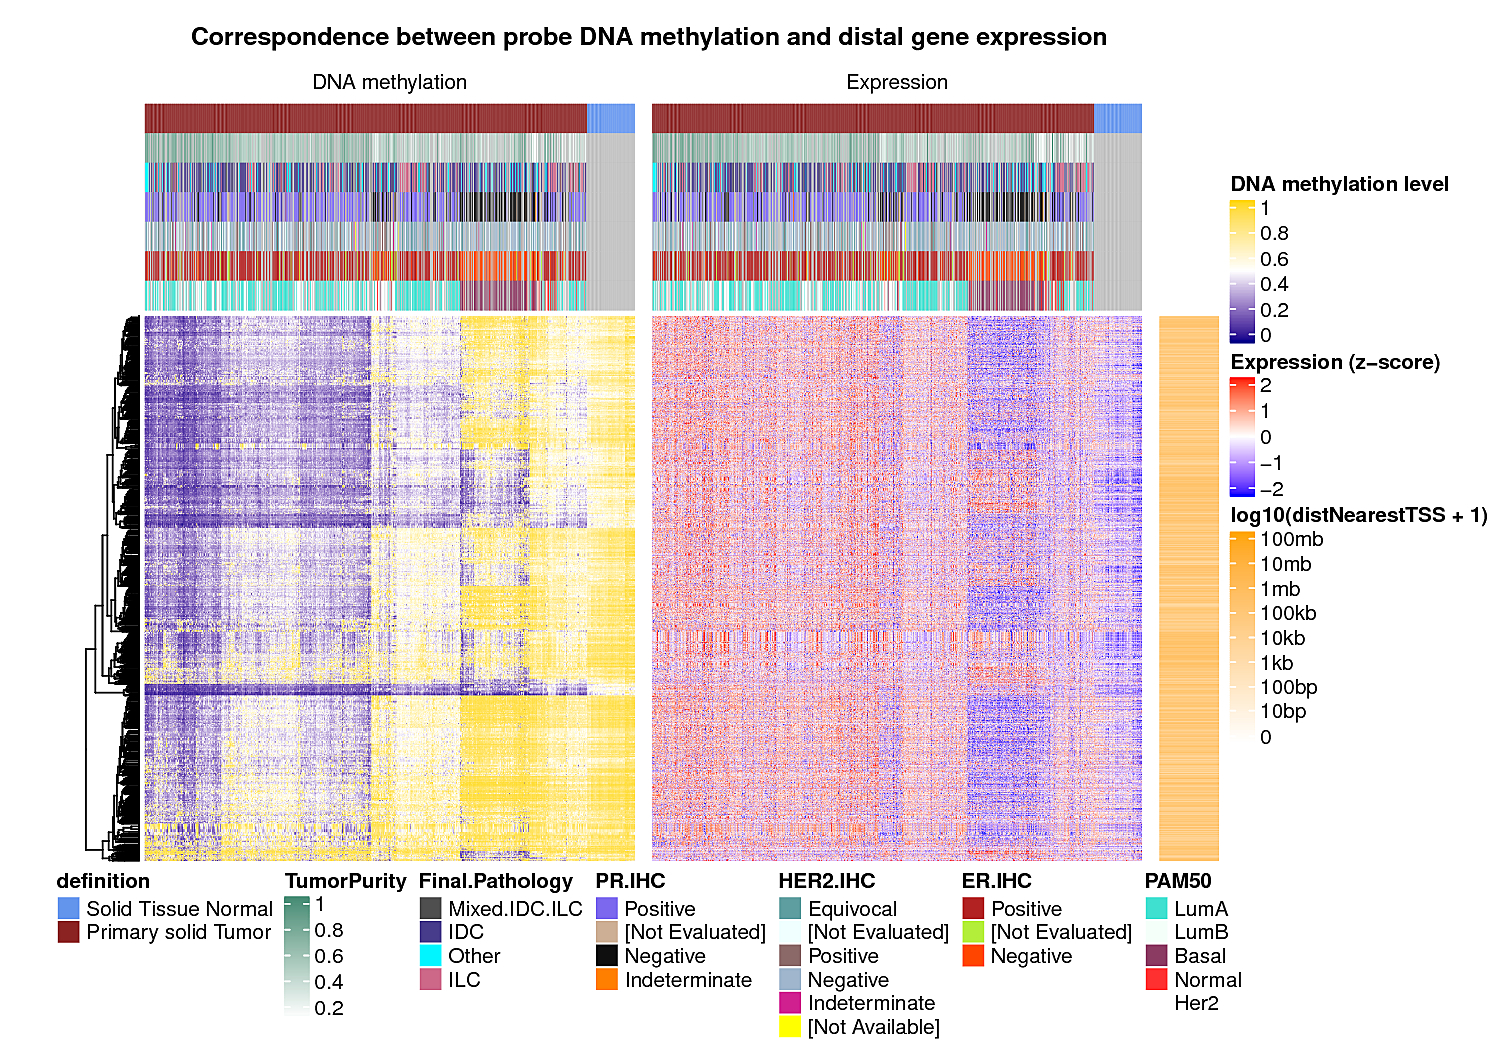
\includegraphics[width=1.0\textwidth]{images/heatmap.jpg}
\caption{\label{fig:heatmap} The comprehensive heatmap view shows all probe / gene pairs identified by ELMER, clustered according to similarity. This plot is based on the Supervised analysis of LumA vs Basal-like Breast Cancer cases. The inverse correlation between methylation and expression can be observed.}
\end{figure}

The unsupervised analysis of the same sample identified several Luminal type Master Regulators (MRs) such as FOXA1, GATA3, and ESR1. In order to identify MRs for the other subtypes, we created a table  (Table \ref{tbl:TF_molecular}) of candidate MRs identified by each pairwise ELMER run (complete results can be found in the supplemental HTML file described in the Supplementary Methods section). 

Interestingly, several new MRs are identified for the Basal-like group, and these were mostly consistent in comparisons against Luminal and HER2+ subtypes. One group of MRs identified are the \textit{SOX10} and \textit{SOX9} TF signatures. For these signatures, the regulatory TF candidate identified are the \textit{SOX9} (Sry-related HMG box-9) TF and \textit{SOX11} (Sry-related HMG box-11) TF; this correlation between basal-like and SOX11 was recently described by \cite{shepherd2016sox11} and \textit{SOX9} was described by \cite{gong2015foxa1}. Most interestingly, we found KLF5 to be a consistently predicted MR for the Basal-like breast subtype. KLF5 is a master pluripotency factor of embryonic stem cells, and has been associated with a number of different cancers. In breast cancer, it's overexpression has been linked to aggressive, ER-negative and basal-like breast cancers \cite{ben2008embryonic}. % PUBMED ID 18443585

\begin{table}[]
\centering
{\small
\caption{Use case 2 - BRCA supervised analysis: Candidate master regulator TFs (MRs) for each molecular subtype found in a pairwise comparison. This table only includes MRs occurring in multiple pairwise comparisons. For the complete table, please see Supplemental Table \ref{suptbl:TF_molecular} in the supplemental material.}
\label{tbl:TF_molecular}
\begin{tabular}{@{}|c|c|c|c|c|c|c|c|c|@{}}
\midrule
\textit{\textbf{TF}} & \textbf{\begin{tabular}[c]{@{}c@{}}LUMA \\ (vs basal)\end{tabular}} & \textbf{\begin{tabular}[c]{@{}c@{}}LUMB \\ (vs basal)\end{tabular}} & \textbf{\begin{tabular}[c]{@{}c@{}}Basal \\ (vs LumB)\end{tabular}} & \textbf{\begin{tabular}[c]{@{}c@{}}Basal \\ (vs HER2)\end{tabular}} & \textbf{\begin{tabular}[c]{@{}c@{}}HER2 \\ (vs Basal)\end{tabular}} \\ \midrule 
\textit{\textbf{AR}} & x & x &  &  &  \\
\textit{\textbf{BCL11A}} &  &  & x & x &  \\
\textit{\textbf{CEBPB}} &  &  & x & x &  \\
\textit{\textbf{E2F3}} &  &  & x & x &  \\
\textit{\textbf{EMX1}} & x & x &  &  &  \\
\textit{\textbf{ESR1}} & x & x &  &  &  \\
\textit{\textbf{ETV6}} &  &  & x & x &  \\
\textit{\textbf{FOXA1}} & x & x &  &  & x \\
\textit{\textbf{FOXP1}} & x & x &  &  & x \\
\textit{\textbf{GATA3}} & x & x &  &  & x \\
\textit{\textbf{GLI1}} & x & x &  &  &  \\
\textit{\textbf{HOXB1}} & x & x &  &  &  \\
%\textit{\textbf{HOXB2}} & x & x &  &  & x \\
\textit{\textbf{HOXB3}} &  &  &  &  & x \\
%\textit{\textbf{HOXB6}} &  &  &  &  & x \\
\textit{\textbf{HOXC10}} &  &  &  &  & x \\
%\textit{\textbf{HOXC11}} &  &  &  &  & x \\
\textit{\textbf{KLF5}} &  &  & x & x &  \\
\textit{\textbf{LMX1B}} & x & x &  &  &  \\
\textit{\textbf{NR2E3}} & x & x &  &  &  \\
%\textit{\textbf{PATZ1}} &  & x &  &  &  \\
\textit{\textbf{PBX1}} &  & x &  &  &  \\
\textit{\textbf{RARA}} & x & x &  &  &  \\
%\textit{\textbf{RUNX3}} &  &  & x &  &  \\
\textit{\textbf{SOX8}} &  &  & x & x &  \\
\textit{\textbf{SOX9}} &  &  & x & x &  \\
\textit{\textbf{SOX11}} &  &  & x &  &  \\
\textit{\textbf{ZNF467}} & x & x &  &  &  \\
\textit{\textbf{ZIC1}} &  &  & x & x &  \\  \hline 
\end{tabular}
}
\end{table}

